\chapter{Pose-Rectified Performance Metrics}
\label{sec:metrics}

\paragraph{Why not a single CLIP alignment score.} Prompt alignment for T2I
generation is usually scored with CLIPScore~\cite{clipscore}: a single cosine
between the generated image and the text prompt in a \emph{pretrained encoder's}
embedding space. For face rotation this one number is insufficient---it
\emph{entangles} every axis of the generation: a CLIP score cannot separate a
wrong \emph{pose} from a wrong \emph{scene} or a lost \emph{identity}, and in
particular cannot say \emph{whether} the requested head turn actually happened
(Fig.~\ref{fig:clipfail})---precisely the distinction our task hinges on. We
want a metric that says \emph{why}.
% --- CLIPScore failure panel (built by figures/make_metric_fail_figs.py) ---
\begin{figure}[t]\centering
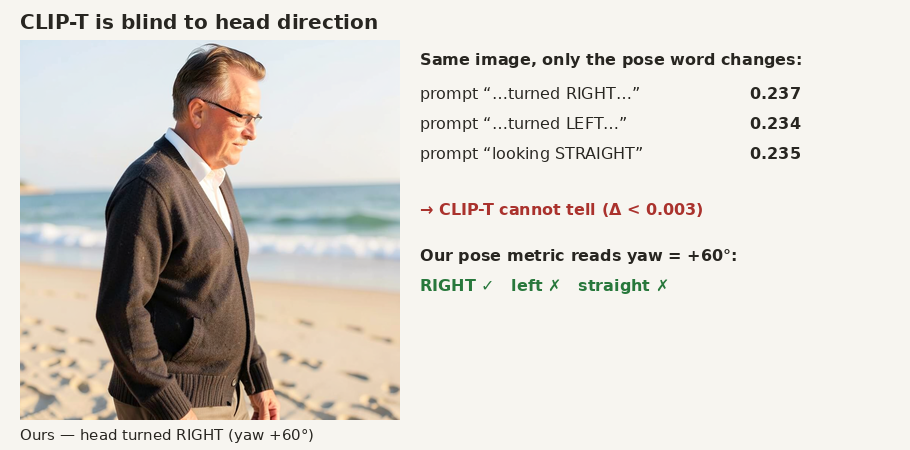
\includegraphics[width=\linewidth]{figures/clip_fail.png}
\caption[CLIPScore is blind to head direction]{\textbf{CLIPScore is blind to head direction.} For a single Rotate-ID
generation whose head is turned right ($\theta_y{=}{+}60^\circ$), CLIP-T against
the \emph{same} prompt with only the pose word changed is essentially constant
(right $0.237$, left $0.234$, straight $0.235$; $\Delta<0.003$): CLIPScore cannot
tell which way---or whether---the head turned. Our estimator-based metric reads
$\theta_y$ directly and verifies the instruction (right~\checkmark, left/straight
$\times$).}
\label{fig:clipfail}
\end{figure}

\paragraph{Expert-decomposed evaluation.} We decompose each generation into the
two axes that define the task and read each one out with a dedicated
\emph{expert} model, rather than a general-purpose encoder
(Fig.~\ref{fig:scoring}):
\begin{itemize}[leftmargin=1.2em,itemsep=2pt,topsep=2pt]
  \item \textbf{Identity ($\mathcal{S}_{\mathrm{id}}$).} We read identity with
  two complementary recognizers from two lines of work---both \emph{existing},
  off-the-shelf encoders, adopted rather than trained---and report them side
  by side: the community-standard, frontal-trained AdaFace
  ir-101~\cite{adaface}, and \textbf{Pose-Adapted face Encoders (PAEs)}
  adapted from PASL~\cite{pasl}, a bank of yaw-routed recognizers
  (full definition in App.~\ref{sec:appendix_profile}). Both read the
  cosine similarity (\csim) between the generated face and the reference under
  MTCNN~\cite{mtcnn} alignment. The
  pairing is deliberate: AdaFace \emph{under}-reads identity at large yaw
  while PAEs are pose-robust, so their gap separates the metric artifact from
  a true identity loss.
  \item \textbf{Pose ($\mathcal{S}_{\mathrm{pose}}$).} A 3D head-pose
  expert (SMPLest-X~\cite{smplestx}) estimates head yaw and pitch from the
  generated image; we compare against the \emph{target} pose and report
  \emph{direction accuracy} for yaw and pitch separately (left/right/forward and
  up/down), so a mistake is attributable to a specific axis rather than a blurred
  similarity.
\end{itemize}

\begin{figure}[!t]\centering
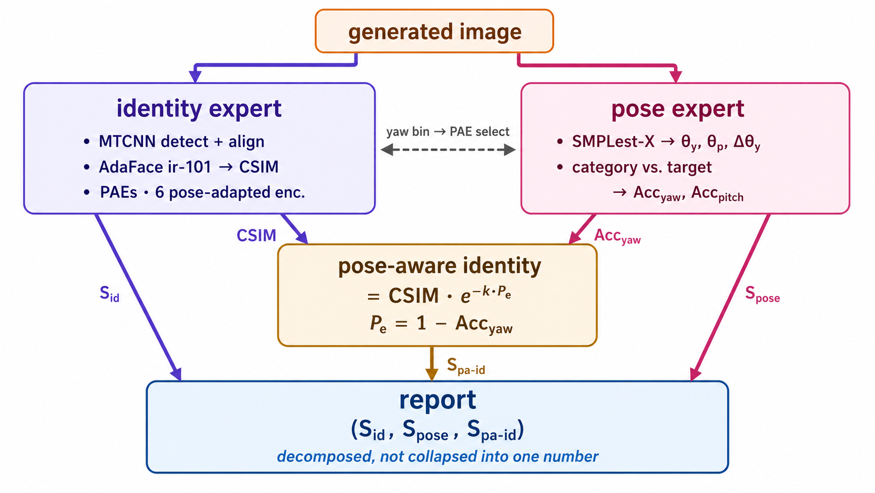
\includegraphics[width=\linewidth]{figures/rotate_id_eval.png}
\caption[The pose-rectified scoring pipeline]{\textbf{The pose-rectified scoring pipeline.} Two dedicated experts
read each generation: the \textbf{pose expert} (SMPLest-X) maps measured angles
to a pose category and checks it against the request
($\mathcal{S}_{\mathrm{pose}}$); the \textbf{identity expert} aligns the face
and reads AdaFace plus the yaw-routed PAEs ($\mathcal{S}_{\mathrm{id}}$). The two
combine into the pose-aware identity $\widetilde{\mathrm{CSIM}}$
(Eq.~\ref{eq:posepenalty}); the report is the decomposed triple
$(\mathcal{S}_{\mathrm{pose}},\widetilde{\mathrm{CSIM}},\mathcal{S}_{\mathrm{id}})$,
so a failure is attributable to a specific axis.}
\label{fig:scoring}
\end{figure}

\paragraph{Pose angles from SMPLest-X.}
We read head and torso orientation in the camera frame by fitting SMPL-X with
SMPLest-X~\cite{smplestx} to the most prominent person, calibrated so that
$0^\circ$ is an upright torso facing the camera ($+$yaw $=$ looking camera-right,
$+$pitch $=$ chin up). Head yaw $\theta_y$ and pitch $\theta_p$ are read from the
head's global rotation (composed along the SMPL-X spine chain, gimbal-safe);
the \emph{head-to-torso yaw} $\Delta\theta_y$---the over-the-shoulder cue---is
the signed angle between the head's and the torso's forward normals in the
horizontal plane, large exactly when the head is turned far relative to the
chest. Exact formulas and calibration constants are in
App.~\ref{sec:appendix_angles}.

\paragraph{Pose-category realization.} Rather than scoring a continuous angle
error---which a single frontal reference cannot calibrate---the pose metric is
\emph{categorical}: each generation is mapped to the same discrete
instructions the prompt uses. Category boundaries were set by annotating a
corpus of real-world portraits with the angles above and locating where a turn
becomes perceptually unambiguous: \emph{turned right} if
$\theta_y\!>\!15^\circ$, \emph{turned left} if $\theta_y\!<\!-15^\circ$ (else
frontal); \emph{over the shoulder} if $|\Delta\theta_y|\!>\!25^\circ$;
\emph{chin up} if $\theta_p\!>\!15^\circ$, \emph{chin down} if
$\theta_p\!<\!-15^\circ$. We check whether each clause of the prompt's
instruction is realized and report per-axis accuracy (yaw, pitch) and their
conjunction (overall pose): a failure names its axis---the head turned the
wrong way, or stayed frontal---an attribution no encoder-space distance
provides.

\paragraph{Pose-aware identity.} Raw \csim{}---under either encoder---rewards
a method for \emph{looking like} the reference even when it ignores the
requested pose: a model that stays near-frontal scores highly while solving
only the easier half of the task. We therefore discount \csim{} by the missed
rotation into a \textbf{pose-aware identity},
\begin{equation}
\widetilde{\mathrm{CSIM}}(k)=\mathrm{CSIM}\cdot e^{-k\,P_e},\qquad
P_e=1-\mathrm{Acc_{yaw}}\in[0,1],
\label{eq:posepenalty}
\end{equation}
where $\mathrm{Acc_{yaw}}$ is the yaw direction accuracy above and $k$ sets
the penalty strength: $k{=}0$ returns the raw score, and a method that never
turns is attenuated by $e^{-k}$. The penalty is tied to \emph{yaw alone} by
design: the out-of-plane turn \emph{is} the rotation the task asks for,
whereas pitch is easier to realize and far less diagnostic; averaging the two
would let weak yaw control hide behind easy pitch
(App.~\ref{sec:appendix_pe} confirms the method ranking also holds under equal
yaw/pitch weighting). The principle is explicit---\emph{identity only counts
at the pose actually requested}---so frontal collapse can no longer masquerade
as identity preservation; we sweep $k$ across methods in
Sec.~\ref{sec:exp_penalized}.

Every method is then scored as the triple
$(\mathcal{S}_{\mathrm{pose}},\,\widetilde{\mathrm{CSIM}},\,
\mathcal{S}_{\mathrm{id}})$---pose accuracy, pose-aware identity, and raw
identity, the identity entries each under both AdaFace and PAEs---plus the
face-detection rate. A weighted scalar is possible, but the value of the
metric is the \emph{decomposition}: a drop in $\mathcal{S}_{\mathrm{id}}$ at
high $\mathcal{S}_{\mathrm{pose}}$ is exactly the profile-view identity loss
we study, and is invisible to a single CLIPScore. The decomposition also
supports \emph{conditional} read-outs---e.g.\ \csim{} as a function of how
many pose criteria were met---which Sec.~\ref{sec:exp} uses to localize
\emph{where} identity is lost; aggregate cross-method scores are reported in
Tables~\ref{tab:sota_pose} and~\ref{tab:posepenalized}.
